\documentclass[11pt,a4paper]{article}

\usepackage[margin=2.6cm]{geometry}
\usepackage{amsmath,amssymb}
\usepackage{graphicx}
\usepackage{xcolor}
\usepackage{tikz}
\usetikzlibrary{arrows.meta,calc,decorations.pathmorphing}
\usepackage{microtype}
\usepackage[hidelinks]{hyperref}

\graphicspath{{../gallery/}}
\setlength{\parskip}{0.55em}
\setlength{\parindent}{0pt}
\linespread{1.08}

% A boxed aside: optional detail for the curious, safe to skip.
\definecolor{asideborder}{RGB}{140,160,200}
\definecolor{asidefill}{RGB}{244,247,252}
\newenvironment{aside}[1]
  {\par\medskip\noindent\begin{center}\begin{tikzpicture}\node[draw=asideborder,fill=asidefill,rounded corners=3pt,inner sep=9pt,text width=0.9\linewidth]\bgroup\small\textbf{#1}\par\smallskip}
  {\egroup;\end{tikzpicture}\end{center}\medskip}

\newcommand{\dd}{\mathrm{d}}
\newcommand{\vect}[1]{\mathbf{#1}}

\title{\textbf{Painting with Light Through a Spinning Black Hole}\\[0.4em]
\large How the simulator draws what it draws}
\author{Alexander Higgins \quad\textperiodcentered\quad written with Claude\\[0.3em]
\small\url{https://github.com/captainchapster/spacetime}}
\date{October 2026}

\begin{document}
\maketitle

\begin{abstract}
\noindent
Every picture the simulator shows is made the way a camera makes one: from light that
reached it. The difference is that the light has travelled through the curved spacetime of
a spinning black hole, so it doesn't go in straight lines. This paper follows a single ray
of light from a pixel on your screen, backwards in time, out past the black hole to wherever
it came from: the glowing disk of gas, the stars of the Milky Way, or nowhere at all. Along
the way we meet the Kerr metric that describes a rotating black hole, Hamilton's equations
(the same ones from classical mechanics) steering the light, the blackbody physics that
colours the gas, and the photographic tricks that turn it all into an image. Nothing beyond
university calculus, linear algebra and a little Hamiltonian mechanics is assumed. Where
the full machinery of general relativity would usually be wheeled in, we will try to make
do with intuition and a few honest equations.
\end{abstract}

\begin{figure}[h]
  \centering
  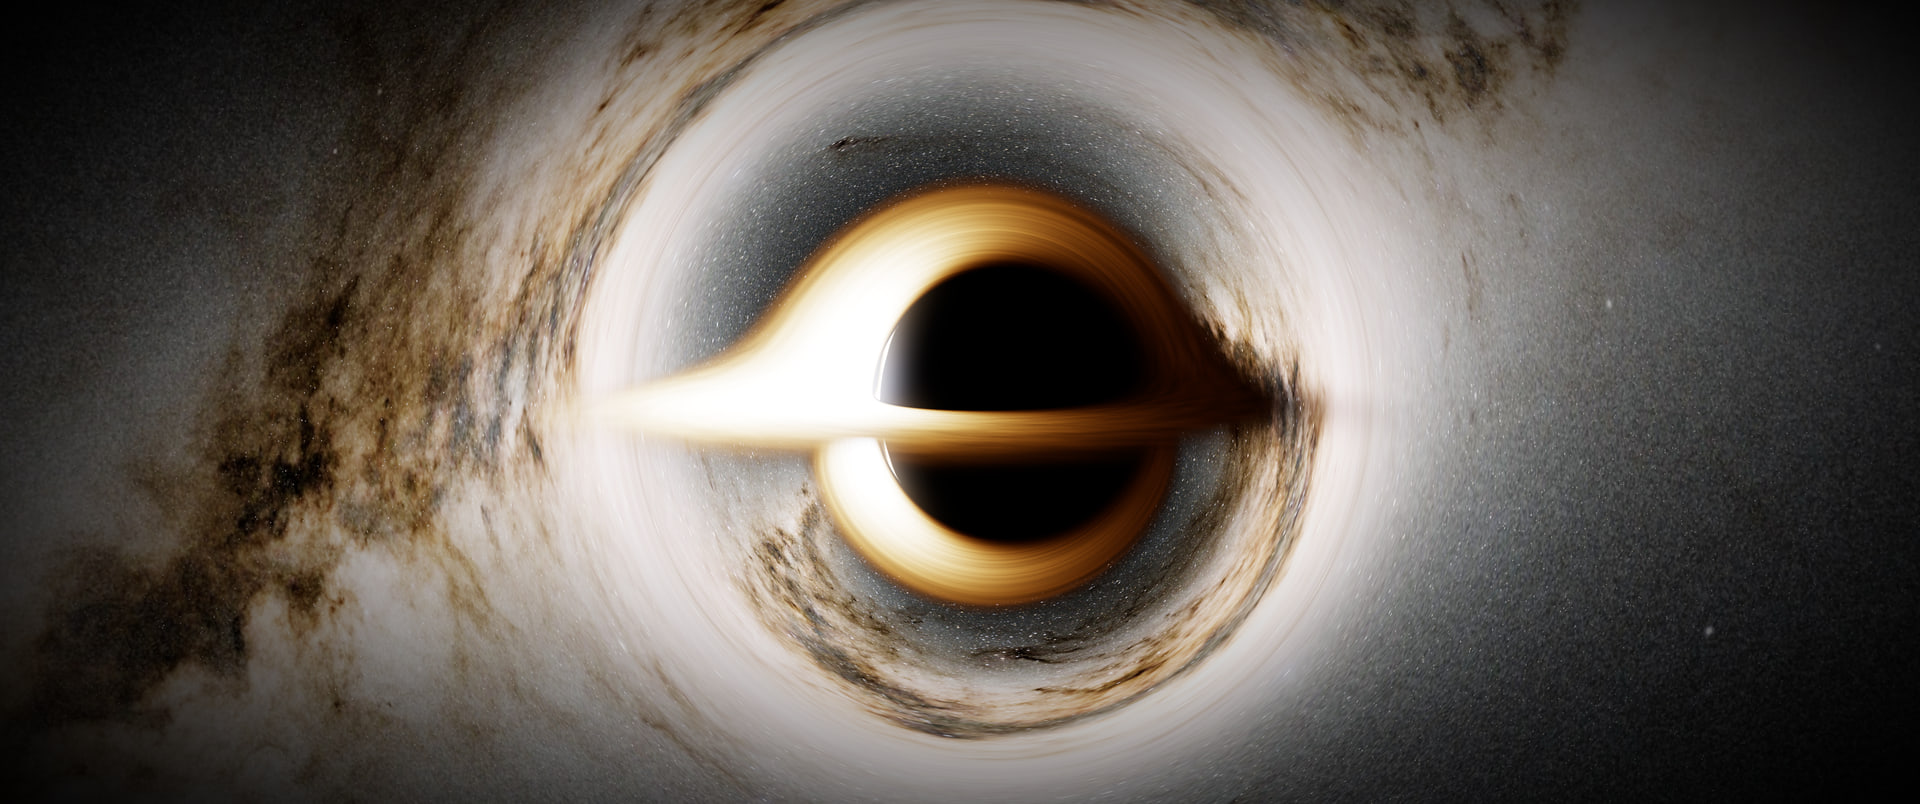
\includegraphics[width=\linewidth]{einstein-ring.jpg}
  \caption{A spinning black hole rendered by the simulator. The black disc is the hole's
  \emph{shadow}; the bright band is the accretion disk, whose far side is lifted into view
  above and below the shadow by the bending of light; the Milky Way behind is bent into a
  ring around it all.}
\end{figure}

\newpage
\begingroup\setlength{\parskip}{0pt}\tableofcontents\endgroup
\newpage

%=======================================================================================
\section{A picture is a collection of light rays}

Look at anything around you. What your eye actually receives is light: a great many rays,
each arriving from a slightly different direction, each carrying a colour and a brightness.
A photograph records the same thing: one pixel, one direction, one colour.

So to draw a black hole we don't need to know what a black hole ``looks like''. We need to
answer, for every pixel, a much more concrete question:
\begin{center}
\emph{If light arrived at the camera from this direction, where did it come from?}
\end{center}
In ordinary space the answer is easy: follow a straight line backwards until it hits
something. Near a black hole, light doesn't travel in straight lines. The black hole curves
spacetime itself, and light simply follows the straightest path the curved geometry
allows. Following that path backwards is called \emph{ray tracing}, and it is all the
simulator really does. Everything you see (the shadow, the ring of light around it, the
disk folded up over the top, the stretched-out stars) falls out of tracing rays correctly;
none of it is painted on.

Why trace \emph{backwards}? Because almost all the light in the universe never reaches the
camera. Tracing forwards from every star and every piece of glowing gas would waste nearly
all the effort on light that goes somewhere else. Tracing backwards from the camera only
ever follows rays that matter. The laws of motion for light don't care about the direction
of time, so following a ray backwards is just as honest as following it forwards.

\begin{figure}[h]
\centering
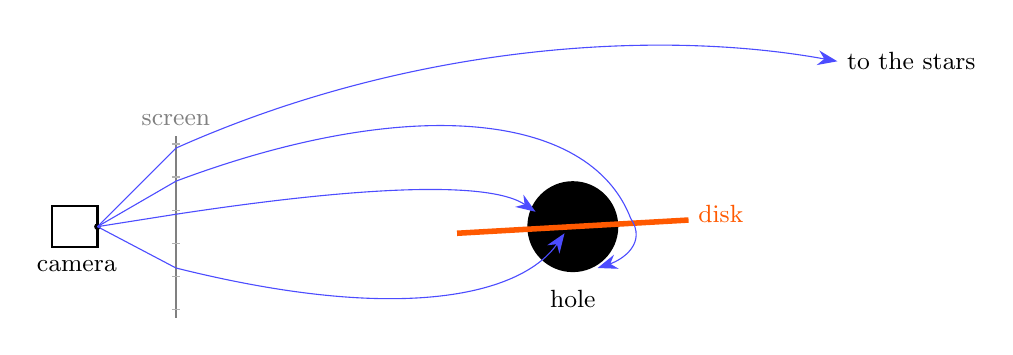
\begin{tikzpicture}[scale=1.05]
  % camera and screen
  \draw[thick] (-0.3,-0.25) rectangle (0.25,0.25);
  \fill (0.25,0) circle (0.04);
  \node[below] at (0,-0.3) {\small camera};
  \draw[gray] (1.2,-1.1) -- (1.2,1.1);
  \foreach \y in {-1.0,-0.6,...,1.0} \draw[gray!60] (1.15,\y) -- (1.25,\y);
  \node[gray,above] at (1.2,1.1) {\small screen};
  % hole
  \fill[black] (6,0) circle (0.55);
  \draw[orange!70!red, line width=2pt] (4.6,-0.08) -- (7.4,0.08);
  % rays
  \draw[-{Stealth[length=2.5mm]}, blue!70] (0.25,0) -- (1.2,0.15) .. controls (3.5,0.5) and (5.0,0.55) .. (5.55,0.18);
  \draw[-{Stealth[length=2.5mm]}, blue!70] (0.25,0) -- (1.2,0.55) .. controls (4.0,1.6) and (6.2,1.4) .. (6.7,0.1) .. controls (6.9,-0.2) and (6.6,-0.4) .. (6.3,-0.5);
  \draw[-{Stealth[length=2.5mm]}, blue!70] (0.25,0) -- (1.2,0.95) .. controls (4,2.2) and (7,2.4) .. (9.2,2.0);
  \draw[-{Stealth[length=2.5mm]}, blue!70] (0.25,0) -- (1.2,-0.5) .. controls (4,-1.2) and (5.4,-0.8) .. (5.9,-0.08);
  \node[right] at (9.2,2.0) {\small to the stars};
  \node[below] at (6,-0.65) {\small hole};
  \node[right,orange!70!red] at (7.4,0.15) {\small disk};
\end{tikzpicture}
\caption{Backward ray tracing. From the camera, one ray is sent out through each pixel and
followed through curved spacetime until it reaches the disk, the distant sky, or the black
hole itself. Rays that pass close to the hole can bend round and hit the far side of the
disk: that is why the disk appears folded over the top of the shadow.}
\end{figure}

The rest of this paper follows one of those rays. We'll need four ingredients:
\begin{enumerate}
  \item a description of the curved spacetime (Section~\ref{sec:spacetime} and
        \ref{sec:kerr});
  \item the law that moves light through it (Section~\ref{sec:motion});
  \item what the ray finds at the end, and what colour that makes the pixel
        (Sections~\ref{sec:ends}--\ref{sec:sky});
  \item the photographic steps that turn physical light into a picture on a screen
        (Section~\ref{sec:photo}).
\end{enumerate}

%=======================================================================================
\section{Spacetime and its ruler}\label{sec:spacetime}

\subsection{Distance in four dimensions}

In ordinary three-dimensional space, Pythagoras tells us the distance between two nearby
points:
\begin{equation}
  \dd s^2 = \dd x^2 + \dd y^2 + \dd z^2 .
\end{equation}
Special relativity adds time as a fourth direction, with a twist: time enters with the
opposite sign. Measuring time in metres (by multiplying seconds by the speed of light, so
that one ``metre of time'' is the time light takes to cross a metre), the
\emph{spacetime interval} between two nearby events is
\begin{equation}
  \dd s^2 = -\dd t^2 + \dd x^2 + \dd y^2 + \dd z^2 .
  \label{eq:minkowski}
\end{equation}
That minus sign is the whole of special relativity in one character. It makes the interval
zero along the path of light: a light ray moving at speed one travels one metre of space
per metre of time, so $\dd x^2 = \dd t^2$ and $\dd s^2 = 0$. Light rays are the paths of
zero interval. Keep that in mind; it is the single most useful fact in this paper.

\subsection{The metric: a matrix that measures}

We can write (\ref{eq:minkowski}) as a matrix product. Collect the four coordinates into a
vector $\dd x^\mu = (\dd t, \dd x, \dd y, \dd z)$ with $\mu = 0,1,2,3$, and put the signs
into a diagonal matrix
\begin{equation}
  \eta_{\mu\nu} = \begin{pmatrix} -1 & 0 & 0 & 0\\ 0 & 1 & 0 & 0\\ 0 & 0 & 1 & 0\\ 0 & 0 & 0 & 1 \end{pmatrix}.
\end{equation}
Then $\dd s^2 = \sum_{\mu,\nu} \eta_{\mu\nu}\, \dd x^\mu \dd x^\nu$. Physicists drop the
summation signs and agree that any index appearing once up and once down is summed over
(Einstein's convention), so this is written
\begin{equation}
  \dd s^2 = \eta_{\mu\nu}\, \dd x^\mu\, \dd x^\nu .
\end{equation}
The matrix $\eta_{\mu\nu}$ is the \emph{metric} of flat spacetime: the ruler that turns
small steps in coordinates into physical intervals.

Gravity, in Einstein's theory, is nothing more than this ruler changing from place to
place. Near a mass, the metric is no longer the simple $\eta_{\mu\nu}$ but some other
symmetric matrix $g_{\mu\nu}(x)$ whose entries depend on where you are:
\begin{equation}
  \dd s^2 = g_{\mu\nu}(x)\, \dd x^\mu\, \dd x^\nu .
\end{equation}
Clocks tick at different rates, rulers stretch, and ``straight lines'' (the paths that
light and falling objects follow) bend. Light still travels along paths with
$\dd s^2 = 0$, but now ``zero'' is measured with the curved ruler.

\begin{aside}{Aside: upstairs and downstairs indices}
You'll see vectors with indices up ($k^\mu$) and down ($p_\mu$). Think of them as column
vectors and row vectors. The metric converts one into the other, $p_\mu = g_{\mu\nu}
k^\nu$, and its matrix inverse $g^{\mu\nu}$ converts back. The ``dot product'' of two
vectors is $g_{\mu\nu}\,a^\mu b^\nu = a^\mu b_\mu$. Nothing deeper is needed here.
\end{aside}

\subsection{Units where the black hole is the ruler}

General relativity is far tidier if we also measure mass in metres, choosing units where
both Newton's constant $G$ and the speed of light $c$ equal one. A mass $M$ then has a
natural length, $GM/c^2$, and a natural time, $GM/c^3$. For the simulator's default black
hole, ``Gargantua'', with a hundred million times the mass of the Sun,
\begin{equation}
  M = \frac{GM}{c^2} \approx 1.48\times 10^{11}\ \text{m} \approx 1\ \text{AU},
  \qquad \frac{GM}{c^3} \approx 493\ \text{s}.
\end{equation}
All distances below are in units of $M$. Saying the event horizon is at $r = 1.31$
therefore means $1.31 \times 1.48\times10^{11}$ metres. The beauty of these units is that
the \emph{shape} of everything (the shadow, the disk, the bending of light) is the same for
every black hole of the same spin; only the scale changes.

%=======================================================================================
\section{The spinning black hole}\label{sec:kerr}

\subsection{Two numbers}

Remarkably, a black hole in empty space is completely described by just two numbers: its
mass $M$ and its spin, usually written $a = J/M$ where $J$ is its angular momentum. (A
third, electric charge, is irrelevant for real black holes.) The spin can range from $0$
(not rotating) up to $a = M$ (the fastest a black hole can spin). The simulator's Gargantua
has $a = 0.95\,M$.

The metric of a spinning black hole was found by Roy Kerr in 1963. It is famously
complicated when written in the usual spherical-looking coordinates, but in a form found by
Kerr and Schild it becomes almost friendly:
\begin{equation}
  \boxed{\,g_{\mu\nu} = \eta_{\mu\nu} + f\, l_\mu\, l_\nu\,}
  \label{eq:ks}
\end{equation}
In words: \emph{flat spacetime plus a correction}, and the correction has a very special
shape, being built from a single four-vector $l_\mu$ multiplied by itself, scaled by a
number $f$. The ingredients are
\begin{align}
  f &= \frac{2 M r^3}{r^4 + a^2 z^2}, \label{eq:f}\\[0.3em]
  l_\mu &= \left(1,\ \frac{r x + a y}{r^2 + a^2},\ \frac{r y - a x}{r^2 + a^2},\ \frac{z}{r}\right). \label{eq:l}
\end{align}
Here $x,y,z$ are ordinary-looking Cartesian coordinates, the spin points along $+z$, and
$r$ is a ``radius'' defined, slightly unusually, by the equation
\begin{equation}
  \frac{x^2 + y^2}{r^2 + a^2} + \frac{z^2}{r^2} = 1 .
  \label{eq:r}
\end{equation}
Surfaces of constant $r$ are not spheres but slightly squashed spheroids, flattened by the
spin. For a non-spinning hole, $a = 0$ and $r$ is just the familiar distance
$\sqrt{x^2+y^2+z^2}$. Equation (\ref{eq:r}) is a quadratic in $r^2$, so $r$ can be found
in closed form:
\begin{equation}
  r^2 = \tfrac12\left(\rho^2 - a^2\right) + \sqrt{\tfrac14\left(\rho^2 - a^2\right)^2 + a^2 z^2},
  \qquad \rho^2 = x^2+y^2+z^2 .
\end{equation}

\begin{aside}{Aside: why this form is so convenient}
The vector $l_\mu$ has zero length as measured by the \emph{flat} metric:
$\eta^{\mu\nu} l_\mu l_\nu = 0$. It points along a light ray. That one property makes the
inverse metric (which we need for the equations of motion) just as simple as the metric
itself:
\[
  g^{\mu\nu} = \eta^{\mu\nu} - f\, l^\mu l^\nu, \qquad l^\mu = \eta^{\mu\nu} l_\nu ,
\]
which you can check by multiplying the two matrices together: the cross terms cancel
because $l^\mu l_\mu = 0$. No $4\times4$ matrix inversion is needed anywhere in the
simulator. Kerr--Schild coordinates are also perfectly smooth at the event horizon (the more
common Boyer--Lindquist coordinates blow up there), so rays and ships can cross it without
the numbers misbehaving.
\end{aside}

\subsection{The landmarks}

A few special radii organise everything you see. With the spin along $z$, and writing
$\Delta = r^2 - 2Mr + a^2$:
\begin{itemize}
  \item \textbf{The event horizon}, where $\Delta = 0$:
        $r_+ = M + \sqrt{M^2 - a^2}$, which is $1.31\,M$ for Gargantua. Nothing inside it
        can get out.
  \item \textbf{The ergosphere}, between the horizon and $r = M + \sqrt{M^2 - a^2\cos^2\theta}$
        ($2M$ at the equator). Space is dragged around with the spin so strongly that
        nothing can stand still relative to the distant stars.
  \item \textbf{The photon region}. Light can travel on closed orbits around the hole.
        Light orbiting in the same direction as the spin can circle as close as $1.39\,M$;
        light orbiting against it must stay out at $3.96\,M$. In between, every radius
        hosts some photon orbit, tilted at some angle.
  \item \textbf{The innermost stable circular orbit} (ISCO), $1.94\,M$ for Gargantua.
        Gas can orbit stably outside it; inside it, it spirals in. It is the inner edge of
        the accretion disk.
\end{itemize}

\begin{figure}[h]
\centering
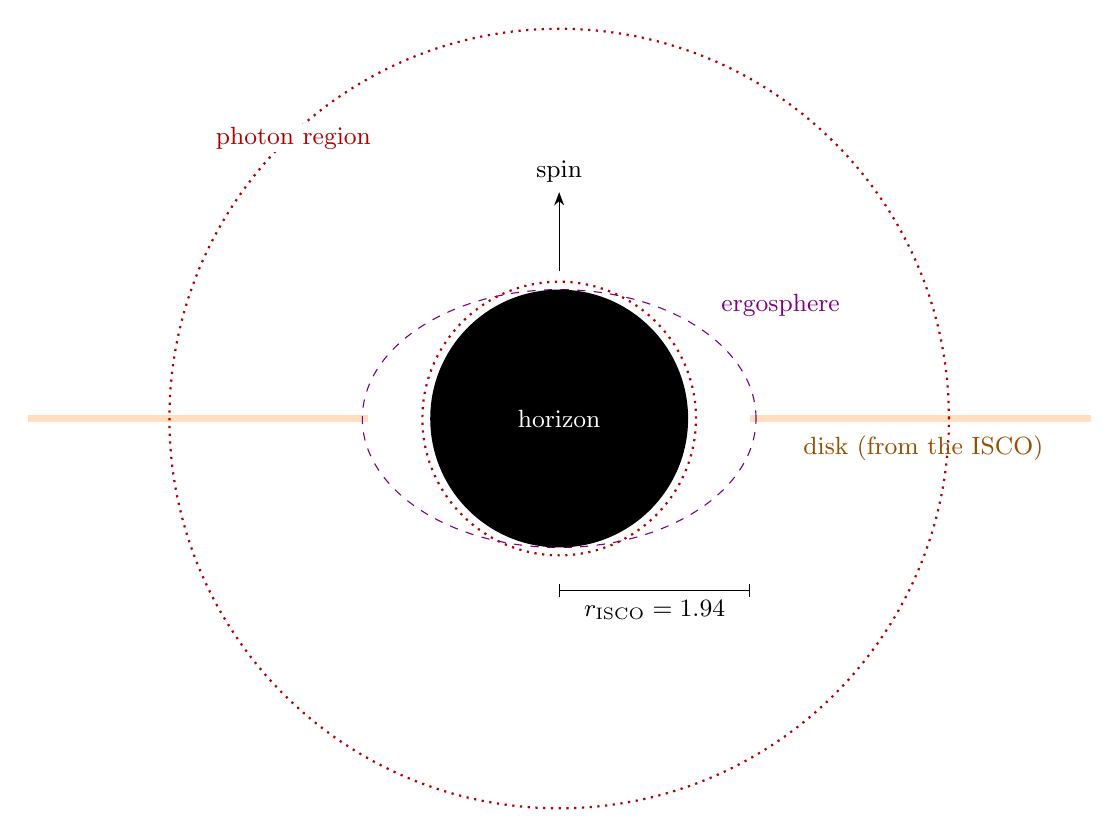
\begin{tikzpicture}[scale=1.25]
  % equatorial cross-section, spin up (z), x horizontal
  \fill[orange!25] (1.94,-0.04) rectangle (5.4,0.04);
  \fill[orange!25] (-1.94,-0.04) rectangle (-5.4,0.04);
  \draw[dashed, violet] (0,0) ellipse (2.0 and 1.31);
  \draw[dotted, thick, red!70!black] (0,0) circle (3.96);
  \draw[dotted, thick, red!70!black] (0,0) circle (1.39);
  \fill[black] (0,0) circle (1.31);
  \draw[-{Stealth}] (0,1.5) -- (0,2.3) node[above] {\small spin};
  \node[white] at (0,0) {\small horizon};
  \node[violet] at (2.25,1.15) {\small ergosphere};
  \node[red!70!black, fill=white, inner sep=1pt] at (-2.7,2.85) {\small photon region};
  \node[orange!60!black] at (3.7,-0.3) {\small disk (from the ISCO)};
  \draw[|-|] (0,-1.75) -- (1.94,-1.75) node[midway,below] {\small $r_{\rm ISCO}=1.94$};
\end{tikzpicture}
\caption{A slice through Gargantua ($a = 0.95\,M$), with equatorial radii to scale. The photon region lies
between the two dotted circles; the disk starts at the ISCO, inside the photon region's
outer edge, which is why so much of the disk light is bent so strongly.}
\end{figure}

%=======================================================================================
\section{How light moves}\label{sec:motion}

\subsection{Hamilton's equations, again}

You have met Hamilton's equations in classical mechanics: a particle's state is a position
and a momentum, and a single function, the Hamiltonian $H(q,p)$, tells you how both evolve,
\begin{equation}
  \frac{\dd q}{\dd\lambda} = \frac{\partial H}{\partial p}, \qquad
  \frac{\dd p}{\dd\lambda} = -\frac{\partial H}{\partial q} .
\end{equation}
Remarkably, the path of light in curved spacetime obeys exactly these equations. The
``position'' is the four coordinates $x^\mu$, the ``momentum'' is the light's four-momentum
$p_\mu$ (energy and ordinary momentum together), the role of time is played by a parameter
$\lambda$ that simply labels points along the ray, and the Hamiltonian is
\begin{equation}
  H = \tfrac12\, g^{\mu\nu}(x)\, p_\mu\, p_\nu .
  \label{eq:H}
\end{equation}
That is the squared length of the momentum, measured with the curved ruler. For light it is
zero, $H = 0$, the same statement as $\dd s^2 = 0$. The equations of motion
\begin{equation}
  \frac{\dd x^\mu}{\dd\lambda} = g^{\mu\nu} p_\nu, \qquad
  \frac{\dd p_\mu}{\dd\lambda} = -\tfrac12\, \frac{\partial g^{\alpha\beta}}{\partial x^\mu}\, p_\alpha\, p_\beta
  \label{eq:hamilton}
\end{equation}
trace out what relativists call a \emph{null geodesic}: the straightest possible path of
zero length. In flat spacetime $g^{\mu\nu}$ is constant, so the momentum never changes and
the ray is a straight line, as it should be. Near a black hole the metric varies from place
to place, the right-hand side of the second equation is not zero, and the ray bends.

Inserting the Kerr--Schild form (\ref{eq:ks}) gives something compact enough to write in
full. Let $L = l^\mu p_\mu$ (one number: how much of the momentum lies along the special
direction $l$). Then
\begin{equation}
  H = \tfrac12\,\eta^{\mu\nu} p_\mu p_\nu \;-\; \tfrac12\, f\, L^2 ,
\end{equation}
flat space plus a single correction, and Hamilton's equations become
\begin{equation}
  \frac{\dd x^\mu}{\dd\lambda} = \eta^{\mu\nu}p_\nu - f L\, l^\mu, \qquad
  \frac{\dd p_i}{\dd\lambda} = \tfrac12\, \frac{\partial f}{\partial x^i}\, L^2 + f L\, \frac{\partial L}{\partial x^i}.
\end{equation}
These eight equations are the heart of the renderer. The derivatives of $f$ and $l_\mu$
are worked out by hand (through the chain rule on $r$, using (\ref{eq:r})) rather than
estimated numerically, because the graphics card works in single precision and numerical
derivatives would be too noisy.

\begin{aside}{Aside: a free conserved quantity}
None of $f$, $l_\mu$ or $r$ depends on the time coordinate $t$. Hamilton's second equation
then says $\dd p_t/\dd\lambda = 0$: the component $p_t$ is constant along every ray. This
is the light's \emph{energy as measured from far away}, and its conservation is what lets
us compute redshifts at the end of the journey without tracking anything extra
(Section~\ref{sec:colour}).
\end{aside}

\subsection{Starting a ray from a pixel}

To begin, we need the camera. The ship carrying it moves with a four-velocity $u^\mu$ and
has three perpendicular axes: right, up and forward, $e_1, e_2, e_3$. Together these four
vectors form the camera's own little patch of flat spacetime, in which the camera sees
exactly what an ordinary camera would. A pixel at screen position $(s_x, s_y)$ corresponds
to the direction
\begin{equation}
  \vect d = \frac{s_x\, e_1 + s_y\, e_2 + e_3}{\left|\,s_x\, e_1 + s_y\, e_2 + e_3\right|},
\end{equation}
with the screen scaled by the field of view. The light arriving from that direction was
travelling \emph{towards} the camera, so to trace it backwards we start with the momentum
\begin{equation}
  k^\mu = -u^\mu + d^\mu ,
\end{equation}
one unit backwards in the camera's time plus one unit out along the pixel's direction. It
has zero length (light-like), and it is normalised so that the camera itself measures the
light's energy as exactly one. Lowering the index with the metric gives the starting
$p_\mu$. Because the camera's own motion is built into $u^\mu$ and $e_i$, the aberration
and Doppler shift caused by the ship's speed come out of this automatically: a ship moving
at $0.9c$ sees the sky crowd towards its direction of travel, with no special code to make
that happen.

\subsection{Stepping along the ray}

Equations (\ref{eq:hamilton}) can't be solved in closed form for a general ray, so they are
integrated numerically with the classical fourth-order Runge--Kutta method: from the
current state, take four trial evaluations of the derivatives across one step, and combine
them so that the error is of fifth order in the step size (Appendix~\ref{app:rk4}).

The art is in choosing the step. Far from the hole, space is nearly flat and a ray barely
bends, so big steps are safe; close to the hole, the ray can swing round in a fraction of
$M$. The simulator scales the step $h$ in $\lambda$ with the distance from the hole, and
shrinks it near the horizons:
\begin{equation}
  h = s \cdot r \cdot n(r)\cdot F(r) \,/\, v ,
\end{equation}
where $s$ is a quality setting (0.03 by default), $n(r)$ falls from 1 to $0.08$ as the ray
approaches a horizon, $F(r)$ allows up to eight times longer steps far away, and $v$
measures how fast the ray is moving through the coordinates, so that each step covers a
similar fraction of the local scale.

\begin{aside}{Aside: light that stands still}
At the outer surface of the ergosphere something odd happens in these coordinates: a ray
can momentarily have almost no motion through \emph{space}, only through time. A step size
set by spatial speed alone would then blow up, and the ray would leap somewhere absurd. In
an early version this appeared as a spray of blue sparkles inside the shadow. The fix is
to bound the step by the ray's motion through time as well: $v$ is the larger of its
spatial speed and half its rate of change of $t$. One honest line, found by tracing the
exact pixel that misbehaved.
\end{aside}

Along the way the simulator checks that $H$ stays close to zero. Integration error can
slowly turn a light ray into something that isn't one; a ray whose $|H|$ has drifted too
far is discarded rather than trusted.

%=======================================================================================
\section{Where rays end}\label{sec:ends}

Every ray eventually meets one of three fates, checked at each step.

\subsection{Out to the stars}

If the ray reaches a large distance (2000\,$M$ or more) and is still moving outward, the
remaining bending is negligible. Its direction of travel there tells us which part of the
sky it came from, and Section~\ref{sec:sky} turns that into a colour.

\subsection{Into the disk}

The accretion disk is modelled as infinitely thin, lying in the equatorial plane $z = 0$
between the ISCO and an outer edge. If the $z$ coordinate of the ray changes sign during a
step, the ray has crossed the plane. Interpolating within the step gives the exact crossing
point, and if its radius lies inside the disk, the ray has found glowing gas. The disk is
partly transparent at its outer rim, so the ray may continue on behind it, adding whatever
it finds there.

\subsection{Into the hole: the shadow}

Some rays have nowhere to come from. Traced backwards, they spiral in toward the horizon.
Forwards in time, that means no light could ever have arrived along them: whatever sent it
would have to be inside the black hole. These pixels are black, and together they form the
\emph{shadow}.

For a non-spinning hole this is easy to picture. Light can orbit the hole at exactly
$r = 3M$, the \emph{photon sphere}. A ray coming in from far away with impact parameter $b$
(how far it would miss the centre if it went straight) is captured if $b$ is less than
\begin{equation}
  b_{\rm crit} = 3\sqrt3\, M \approx 5.196\, M ,
\end{equation}
and escapes otherwise. Rays with $b$ just above the critical value wrap around the hole
once, twice, many times before escaping, which is where the thin, bright \emph{photon ring}
at the edge of the shadow comes from. Notice that the shadow (radius $5.2M$ seen from afar)
is much bigger than the horizon itself ($2M$): the hole's gravity magnifies its own
silhouette.

For a spinning hole the shadow is lopsided, flattened on the side moving towards you,
because light travelling with the spin can approach more closely. The simulator doesn't
need a formula for the shadow's shape; it emerges from tracing the rays. But it does need
to know when to stop following a ray that is doomed, because following a ray all the way
into a horizon is expensive: in these coordinates, a ray approaching the horizon from
outside slows to a crawl and never quite arrives.

\subsection{Knowing a ray is doomed: Carter's constant}

Light moving around a Kerr black hole has three conserved quantities. Two are familiar:
its energy $E = -p_t$, and its angular momentum about the spin axis, $L = x p_y - y p_x$.
The third is a hidden one, discovered by Brandon Carter in 1968, which has no equivalent in
Newtonian gravity:
\begin{equation}
  Q = p_\theta^2 + \cos^2\theta \left( \frac{L^2}{\sin^2\theta} - a^2 E^2 \right).
\end{equation}
(Here $\theta$ is the angle from the spin axis and $p_\theta$ the corresponding momentum.)
With three constants of motion, the radial motion separates from the rest, exactly as it
does for planetary orbits. Its equation is
\begin{equation}
  \left(\Sigma\, \frac{\dd r}{\dd\lambda}\right)^2 = R(r)
  = \big[E\,(r^2 + a^2) - aL\big]^2 - \Delta \big[(L - aE)^2 + Q\big] ,
\end{equation}
where $\Sigma = r^2 + a^2\cos^2\theta$. The left side is a square, so the ray can only be
where $R(r) \ge 0$, and it turns around where $R = 0$. A ray heading inwards will therefore
reach the horizon if, and only if, $R(r)$ stays positive all the way down. The simulator
evaluates $R$ at a few dozen radii between the ray and the horizon. If it is clearly
positive throughout, the ray is captured on the spot. Thousands of integration steps are
saved, and the answer is exact rather than a rule of thumb. (A test in the project checks
the verdict against slow, brute-force integration for rays fired in all directions.)

%=======================================================================================
\section{The glowing gas}\label{sec:disk}

\subsection{An orbiting river of gas}

The disk is gas spiralling slowly inward, each parcel moving on a nearly circular orbit.
For a Kerr black hole the angular velocity of a circular orbit in the equatorial plane is
\begin{equation}
  \Omega(r) = \frac{\sqrt M}{r^{3/2} + a\sqrt M},
\end{equation}
which reduces to Kepler's law $\Omega^2 = M/r^3$ far away. Close to the hole the gas moves
at a large fraction of the speed of light: at Gargantua's ISCO it is about $0.62\,c$
relative to a local observer turning with the dragged space. (Nobody can hover there: it
lies inside the ergosphere.)

Friction between neighbouring rings moving at different speeds (viscosity, ultimately
turbulence) heats the gas, letting it slowly lose energy and drift inward. The energy
released per unit area of disk was worked out by Novikov, Page and Thorne in the 1970s.
Far from the hole their flux reduces to the Newtonian result
\begin{equation}
  F(r) = \frac{3 M \dot M}{8\pi r^3}\left(1 - \sqrt{\frac{r_{\rm in}}{r}}\right),
\end{equation}
where $\dot M$ is the rate at which mass flows in and $r_{\rm in}$ is the inner edge. The
simulator uses the full relativistic version, computed from the exact energies and angular
momenta of circular Kerr orbits. Each patch of disk radiates like a \emph{blackbody}, so its
temperature follows from the Stefan--Boltzmann law:
\begin{equation}
  \sigma T^4 = F .
\end{equation}
With Gargantua's settings (a very gentle inflow, about three ten-millionths of the
``Eddington'' rate at which the light's pressure would balance gravity), the hottest ring sits just outside the ISCO at around 5800\,K, much
like the surface of the Sun. That is why the default disk glows a warm white-gold.

\subsection{The texture}

Real disks are turbulent, so the simulator overlays a pattern of brightness variations
that is carried round at the exact orbital speed of each radius, and seen as it was when
its light left. This pattern is the one artistic element in the disk, and it is labelled
as such. One subtlety: inner rings orbit faster than outer ones, so any fixed pattern
would be sheared into ever-finer spirals and, after a long time warp, look frozen. Real
turbulence keeps renewing itself, so each eddy in the pattern lives about two orbits
before fading into a new one.

%=======================================================================================
\section{Colour: what the light looks like when it arrives}\label{sec:colour}

\subsection{One number for every shift}

Light arriving from the disk has been shifted in frequency, for two reasons. The gas
moving towards you is blueshifted and the gas moving away is redshifted, just as with a
passing siren. And light climbing out of a gravitational well loses energy, so it arrives
redder than it left. In general relativity these aren't separate effects to be added up;
there is a single frequency ratio
\begin{equation}
  g = \frac{\nu_{\rm received}}{\nu_{\rm emitted}}
    = \frac{p_\mu u^\mu_{\rm camera}}{p_\mu u^\mu_{\rm gas}} ,
\end{equation}
the energy of the light measured by the camera divided by its energy measured by the gas
that emitted it. (An observer moving with four-velocity $u^\mu$ measures a photon's energy
as $-p_\mu u^\mu$.) We chose the starting momentum so that the camera's measurement is
exactly one, so the ratio is simply $g = 1/(p_\mu u^\mu_{\rm gas})$, evaluated where the ray
crosses the disk. All of the Doppler shift, the gravitational redshift, and the time
dilation between gas and camera are in this one number.

\subsection{A blackbody stays a blackbody}

Now comes a small miracle. As light travels, the quantity $I_\nu/\nu^3$ is conserved, where
$I_\nu$ is its intensity at frequency $\nu$. (This is Liouville's theorem from Hamiltonian
mechanics: phase-space density is conserved along the flow.) Planck's law for a blackbody
at temperature $T$ reads
\begin{equation}
  I_\nu = \frac{2h\nu^3}{c^2}\, \frac{1}{e^{h\nu/kT} - 1},
  \qquad\text{so}\qquad
  \frac{I_\nu}{\nu^3} = \frac{2h}{c^2}\, \frac{1}{e^{h\nu/kT} - 1},
\end{equation}
which depends on $\nu$ and $T$ only through $\nu/T$. If every frequency is multiplied by
$g$ and $I_\nu/\nu^3$ is unchanged, the received light is \emph{exactly} a blackbody at
temperature $gT$. All the relativity collapses into one substitution,
\begin{equation}
  T_{\rm seen} = g\, T_{\rm gas} ,
\end{equation}
and the total brightness, proportional to $T^4$, changes by $g^4$. That fourth power is why
the side of the disk coming towards you, with $g$ perhaps 1.5, glows $1.5^4 \approx 5$
times brighter than it would at rest, while the receding side fades. It is called
relativistic beaming, and it is why the disk in the images is so lopsided.

\subsection{From temperature to a pixel colour}

The colour of a blackbody at temperature $T$ is computed once and stored in a table:
\begin{enumerate}
  \item Planck's spectrum is weighted by the standard CIE 1931 colour-matching functions,
        the measured sensitivities of the human eye's colour response, giving three
        numbers $X$, $Y$, $Z$ ($Y$ being perceived brightness).
  \item A fixed $3\times 3$ matrix converts $XYZ$ to the red, green and blue of a standard
        sRGB screen.
\end{enumerate}
During rendering, the pixel just looks up the colour at $g\,T_{\rm gas}$. Hot gas is
bluish white, cooler gas orange, and the faint outer disk a deep red, all from physics
rather than a chosen palette.

%=======================================================================================
\section{The sky}\label{sec:sky}

Rays that escape carry a direction on the sky. The simulator offers three skies: a
procedural starfield, a lensing grid (lines of latitude and longitude, to show the
distortion), and the real sky:
\begin{itemize}
  \item \textbf{The Milky Way}: NASA's Deep Star Maps all-sky image, with the stars removed,
        stored as a panoramic texture in galactic coordinates.
  \item \textbf{The stars}: all 117{,}955 stars of the Hipparcos catalogue, each placed at
        its exact position with its own colour (from its measured $B-V$ colour index,
        converted to a temperature).
\end{itemize}
Stars are points, but a pixel covers a small patch of sky, and near the hole that patch can
be hugely magnified or squeezed by lensing. So each pixel measures how much sky it actually
spans, by comparing its escape direction with its neighbours', and adds up the stars
inside that patch. This keeps stars sharp where the sky is magnified and stops them
vanishing between pixels where it is compressed. Starlight is shifted by $g$ too, so the
sky in front of a fast-moving ship turns bluer and brighter.

The most striking result is the \emph{Einstein ring}. A star (or a whole galaxy) exactly
behind the hole is seen not as a point but as a ring, because light from it can pass the
hole on any side. In the opening figure, the Milky Way is bent into exactly such a ring.

%=======================================================================================
\section{From light to a photograph}\label{sec:photo}

At this point each pixel holds a physical brightness: an amount of light in red, green and
blue, which can range over many orders of magnitude between the hot inner disk and a faint
star. A screen can show a range of only about a hundred to one. Turning one into the other
is photography rather than physics, and the simulator says so:
\begin{enumerate}
  \item \textbf{Exposure.} Everything is multiplied by one number, like choosing a
        shutter speed. Automatic exposure adjusts it so the brightest few percent of the
        picture sit near white, as a camera or your eye would.
  \item \textbf{Bloom.} Real lenses scatter a little light from bright sources into a soft
        glow around them. The brightest parts of the image are blurred and added back
        faintly.
  \item \textbf{Tone mapping.} A smooth ``filmic'' curve, the ACES approximation
        \[
          x \;\mapsto\; \frac{x\,(2.51\,x + 0.03)}{x\,(2.43\,x + 0.59) + 0.14},
        \]
        compresses highlights gracefully instead of clipping them to white, much as
        photographic film does.
  \item \textbf{sRGB encoding} adjusts the numbers for how screens display brightness.
\end{enumerate}
Optional film grain, a vignette and colour ``looks'' are available for photographs, and are
labelled as artistic. The disk's turbulence pattern and the brightness of the sky relative
to the disk are the only other artistic choices; the shapes, positions, colours and
relative brightnesses of everything else are computed.

%=======================================================================================
\section{Doing it two million times, sixty times a second}\label{sec:gpu}

A modest window has a couple of million pixels, and each ray needs a hundred or more
Runge--Kutta steps, each needing four evaluations of the equations. That is around a
billion small calculations per frame, far too many for an ordinary processor. But every
pixel's ray is independent of every other, which is exactly the kind of problem a graphics
card is built for: it runs thousands of small programs side by side, one per pixel.

The ray tracer is therefore written as a \emph{fragment shader}, a short program the
graphics card runs for every pixel at once. The same equations are also written out in
ordinary code for the computer's main processor. That copy is used by the sound and the
instruments (which also need to know where light comes from), and by the tests that check
the physics. Keeping the two line-for-line identical means a passing test vouches for the
pixels.

A few economies make it run in real time without changing the picture:
\begin{itemize}
  \item rays are stopped the moment their fate is certain, using Carter's constant as
        described above, but only once nothing else (the disk, a beacon) still lies on
        their way in;
  \item the picture is traced at a fraction of screen resolution and smoothly enlarged,
        with the fraction lowered automatically if frames take too long;
  \item when nothing changes (the simulation is paused, or the journey has ended), no new
        picture is traced at all.
\end{itemize}
Comparing frames before and after these changes, pixel by pixel, the pictures are
identical.

%=======================================================================================
\section{How we know it's right}

A beautiful picture can still be wrong. The simulator's results are checked against exact
results from the literature, through automated tests:
\begin{itemize}
  \item the edges of the shadow agree with the exact critical photon orbits, $3\sqrt3\,M$
        for a non-spinning hole and the known asymmetric values for a spinning one;
        measured in the rendered images themselves, the shadow is the right size to within
        a pixel;
  \item light holds on the photon sphere; captured and escaping rays agree with slow,
        brute-force integration;
  \item the orbital speeds of the disk gas match the classic results of Bardeen, Press and
        Teukolsky (1972);
  \item gyroscopes carried by the ship precess at exactly the Lense--Thirring rates that
        Gravity Probe B measured around the Earth;
  \item inside the horizon, the patch of sky still visible, and its redshift, match the
        exact formulas for a falling observer.
\end{itemize}
A separate set of checks, in Python, builds the curvature of the Kerr--Schild metric with
symbolic algebra and confirms that it satisfies Einstein's equations for empty space (its
Ricci curvature vanishes, to ten decimal places, at sample points around the hole). The
same checks confirm the exact inverse metric and other quantities used above.

%=======================================================================================
\section{Closing thoughts}

It is worth stepping back to see how little was needed. A single matrix, $g_{\mu\nu}$, built
from two numbers, the mass and the spin. A single function, the Hamiltonian, borrowed
unchanged from classical mechanics. One conserved quantity for the energy of light, and one
small miracle about blackbodies. From those, followed faithfully tens of billions of times
a second, come the shadow, the photon ring, the disk lifted over the top of the hole, the
lopsided glow of beaming, and the sky folded into rings.

When the film \emph{Interstellar} rendered its black hole in 2014, the team at Double
Negative and Kip Thorne did essentially this, with the same equations, on a render farm,
over hours per frame. That it can now run live in a web browser, on the graphics card of
an ordinary computer, says less about cleverness than about how kind nature's equations
can be, once you write them the right way.

\subsection*{Further reading}
\begin{itemize}
  \item J.\,B.~Hartle, \emph{Gravity: An Introduction to Einstein's General Relativity}
        (Addison-Wesley, 2003). The gentlest proper introduction; physics first,
        mathematics as needed.
  \item O.~James, E.~von Tunzelmann, P.~Franklin and K.\,S.~Thorne, ``Gravitational
        lensing by spinning black holes in astrophysics, and in the movie
        \emph{Interstellar}'', \emph{Classical and Quantum Gravity} \textbf{32}, 065001
        (2015). How the film's black hole was rendered.
  \item J.-P.~Luminet, ``Image of a spherical black hole with thin accretion disk'',
        \emph{Astronomy and Astrophysics} \textbf{75}, 228 (1979). The first such picture,
        drawn by hand from computer output.
  \item J.\,M.~Bardeen, W.\,H.~Press and S.\,A.~Teukolsky, ``Rotating black holes:
        locally nonrotating frames, energy extraction, and scalar synchrotron radiation'',
        \emph{Astrophysical Journal} \textbf{178}, 347 (1972).
  \item B.~Carter, ``Global structure of the Kerr family of gravitational fields'',
        \emph{Physical Review} \textbf{174}, 1559 (1968).
  \item D.\,N.~Page and K.\,S.~Thorne, ``Disk-accretion onto a black hole: time-averaged
        structure of accretion disk'', \emph{Astrophysical Journal} \textbf{191}, 499
        (1974).
  \item S.~Carroll, \emph{Spacetime and Geometry} (Addison-Wesley, 2004). The next step,
        when you want the full machinery.
\end{itemize}

\appendix
%=======================================================================================
\section{The fourth-order Runge--Kutta method}\label{app:rk4}

Write the state of a ray as $\vect y = (x^\mu, p_\mu)$ and the equations of motion as
$\dd\vect y/\dd\lambda = \vect F(\vect y)$. One step of size $h$ is
\begin{align*}
  \vect k_1 &= \vect F(\vect y), &
  \vect k_2 &= \vect F\!\left(\vect y + \tfrac h2\, \vect k_1\right),\\
  \vect k_3 &= \vect F\!\left(\vect y + \tfrac h2\, \vect k_2\right), &
  \vect k_4 &= \vect F(\vect y + h\, \vect k_3),
\end{align*}
\[
  \vect y \;\to\; \vect y + \frac h6\left(\vect k_1 + 2\vect k_2 + 2\vect k_3 + \vect k_4\right).
\]
It is the numerical cousin of Simpson's rule: the derivative is sampled at the start, twice
in the middle and at the end of the step, and averaged with weights $1{:}2{:}2{:}1$. The
error per step shrinks as $h^5$, so halving the step makes each step about thirty times
more accurate.

\section{Numbers for the default black hole}

\begin{center}
\begin{tabular}{lll}
  \hline
  Quantity & In units of $M$ & For $10^8$ solar masses \\
  \hline
  Unit of length, $GM/c^2$ & 1 & $1.48\times10^{11}$ m (about 1 AU) \\
  Unit of time, $GM/c^3$ & 1 & 493 s \\
  Spin $a$ & 0.95 & \\
  Event horizon $r_+$ & 1.31 & 1.94\,$\times10^{11}$ m \\
  Inner photon orbit (prograde) & 1.39 & \\
  ISCO (disk inner edge) & 1.94 & \\
  Ergosphere (equator) & 2.00 & \\
  Outer photon orbit (retrograde) & 3.96 & \\
  Hottest ring of the disk & 2.8 & about 5800 K \\
  \hline
\end{tabular}
\end{center}

\end{document}
